\section{Agent Prévision : prévoir les rendements, et savoir y renoncer}
\label{sec:prevision}

\subsection{Formulation : une régression sur données temporelles}

L'agent Prévision cherche à repérer les actifs qui feront mieux que les autres le mois suivant. Pour chaque actif $i$ et chaque date $t$, la cible est le rendement \emph{excédentaire} sur $H = 21$ jours de bourse :
\begin{equation}
  y_{i,t} = r_{i,\,t\to t+H} - \frac{1}{N_t}\sum_{j=1}^{N_t} r_{j,\,t\to t+H}.
\end{equation}
Retirer la moyenne des actifs supprime l'effet \og marché \fg{} commun, que l'allocation n'a pas besoin de prévoir : seul compte le classement relatif. La cible a un écart-type de 5,1 \% par mois sur l'entraînement.

Les données sont organisées par \textbf{fenêtre glissante}, comme le présente le cours pour les données temporelles (tableau~\ref{tab:fenetre}). À chaque date, les 31 variables de la section~\ref{sec:donnees} résument le passé, et la cible porte sur l'horizon futur.

\begin{table}[!htb]
  \centering
  \small
  \caption{Paramètres de la fenêtre glissante.}
  \label{tab:fenetre}
  \begin{tabularx}{\textwidth}{@{}l L L@{}}
    \toprule
    \textbf{Terme} & \textbf{Définition} & \textbf{Valeur dans le projet} \\
    \midrule
    \emph{Lookback} $L$ & Nombre de pas passés utilisés en entrée & 252 jours (la variable la plus longue porte sur un an) \\
    \emph{Forecast horizon} $H$ & Nombre de pas futurs à prédire & 21 jours, prévision directe \\
    \emph{Stride} $S$ & Décalage entre deux échantillons & 5 jours (un échantillon par semaine) \\
    \emph{Input size} & Variables par pas de temps & 31 \\
    Chevauchement & Échantillons dont les cibles se recouvrent & $\lceil H/S\rceil - 1 = 4$ \\
    \bottomrule
  \end{tabularx}
\end{table}

Le choix du \emph{stride} est un compromis. Avec $S = 1$, deux échantillons consécutifs partageraient 20 jours de cible sur 21 : ce seraient presque des doublons, qui donneraient une fausse impression de quantité de données. Avec $S = 21$, il ne resterait qu'environ 110 dates d'entraînement. Avec $S = 5$, le chevauchement résiduel de quatre échantillons est pris en compte dans les tests statistiques (correction de Newey-West~\cite{newey1987} et test de Diebold-Mariano). Le panel compte 98\,716 observations ; après découpage et purge, l'entraînement couvre 449 dates (2011-2019), la validation 96 (2020-2021) et le test 241 (janvier 2022 à octobre 2026).

\subsection{Analyse exploratoire du pouvoir prédictif}

En gestion d'actifs, on mesure le pouvoir prédictif d'une variable par son \textbf{coefficient d'information} (IC) : la corrélation de rang de Spearman entre la variable et le rendement futur, calculée date par date puis moyennée. Un IC de 0,03 à 0,05, s'il est stable, est déjà considéré comme exploitable.

Sur l'entraînement, la médiane des IC en valeur absolue n'est que de 0,04. Les variables les plus liées au rendement futur sont la corrélation au S\&P~500 (0,15), le bêta (0,12) et la volatilité (0,07), toutes de signe positif. Elles ne repèrent pas les bons actifs \emph{au sein} d'une classe : elles distinguent les actions des obligations. De 2011 à 2019, marché haussier, les actifs risqués ont nettement battu les actifs défensifs. Ce \og signal \fg{} est une \emph{prime de classe d'actifs propre à la période d'entraînement}. Si le contexte change, il peut disparaître : c'est un risque de \textbf{dérive des données} (\emph{data drift}), et c'est ce qui se produira en 2022.

L'analyse montre aussi que les variables techniques sont fortement corrélées entre elles : différents horizons de momentum, différentes mesures de volatilité. Deux conséquences en découlent : il faudra des modèles régularisés, et une réduction de dimension peut être envisagée.

\subsection{Réduction de dimension : analyse en composantes principales}

L'ACP remplace des variables corrélées par des combinaisons linéaires non corrélées, les composantes principales $F_k = X V_k$, où les $V_k$ sont les vecteurs propres de la matrice de covariance des variables standardisées, rangés par valeur propre $\lambda_k$ décroissante. La part de variance expliquée par $F_k$ vaut $\lambda_k/\sum_j \lambda_j$.

Le cours rappelle que l'ACP n'a d'intérêt que si les variables sont suffisamment corrélées. Nous l'avons vérifié sur l'entraînement : l'indice KMO~\cite{kaiser1974} vaut 0,746 (au-dessus du seuil de 0,6) et le test de sphéricité de Bartlett est très significatif ($\chi^2 = 254\,994$, 190 degrés de liberté, $p < 10^{-4}$). L'ACP est donc justifiée.

\begin{figure}[!htb]
  \centering
  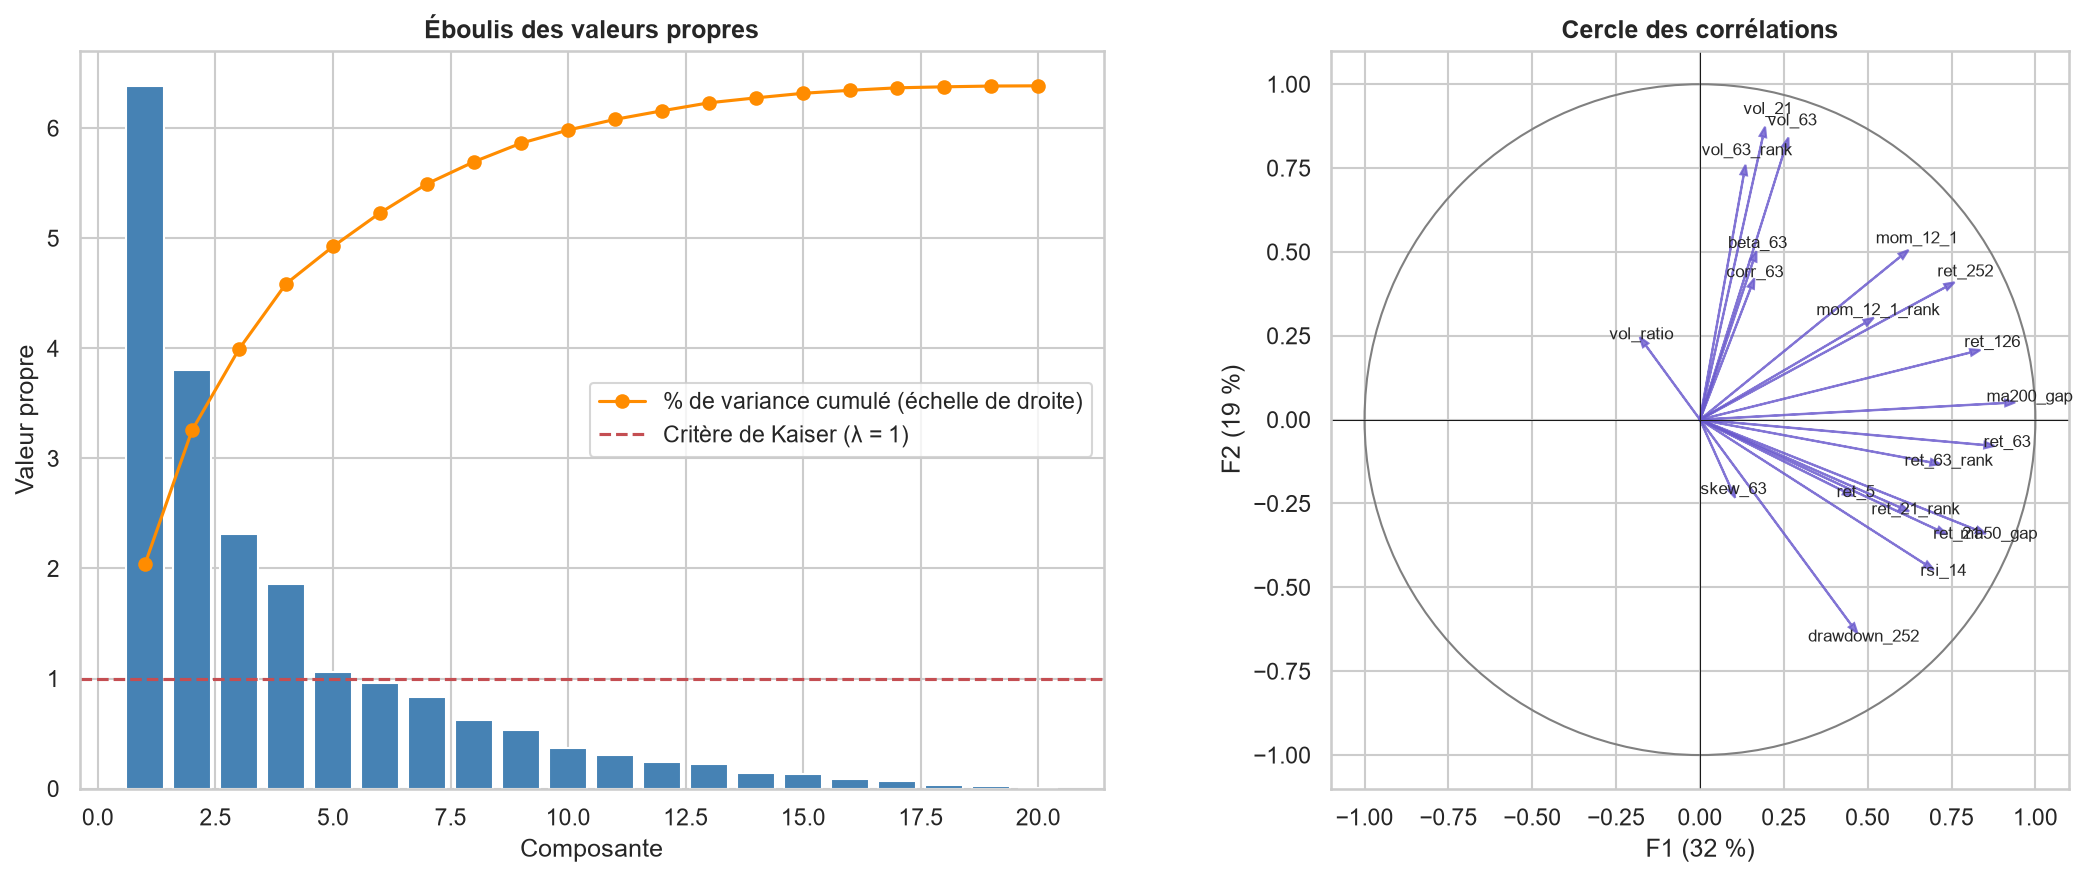
\includegraphics[width=\textwidth]{10b_acp.png}
  \caption{ACP des 20 variables techniques (entraînement) : éboulis des valeurs propres et cercle des corrélations sur le premier plan factoriel.}
  \label{fig:acp}
\end{figure}

Les deux premières composantes expliquent 51 \% de la variance, les cinq premières 77 \% (figure~\ref{fig:acp}). Elles ont une lecture financière claire :
\begin{itemize}
  \item \textbf{F1, \og tendance \fg{}} (32 \%) : corrélée à tous les rendements passés et aux écarts aux moyennes mobiles ;
  \item \textbf{F2, \og risque \fg{}} (19 \%) : corrélée aux volatilités, elle oppose les actifs agités aux actifs calmes ;
  \item \textbf{F3, \og retournement \fg{}} (12 \%) : elle oppose le momentum long au momentum court ;
  \item \textbf{F4, \og sensibilité au marché \fg{}} (9 \%) : corrélée au bêta et à la corrélation au S\&P~500.
\end{itemize}
Les critères de choix du nombre de composantes ne s'accordent pas : 2 selon le coude, 5 selon Kaiser ($\lambda \geq 1$), 6 pour 80 \% de variance, 9 pour 90 \%. Plutôt que de trancher a priori, nous testerons les modèles avec et sans ACP dans le pipeline.

\subsection{Références et modèles comparés}

Toute méthode doit faire mieux que des \textbf{références} sans apprentissage :
\begin{itemize}
  \item la \textbf{prévision nulle}, $\hat y = 0$ : aucun actif ne fera mieux que la moyenne ;
  \item la \textbf{moyenne historique par actif} : le rendement excédentaire moyen de chaque actif sur l'entraînement ;
  \item le \textbf{momentum 12-1} : les gagnants des douze derniers mois (hors le dernier) continuent de gagner.
\end{itemize}

Treize modèles du cours ont été comparés, tous dans un pipeline de prétraitement : régression linéaire (MCO) ; Ridge, Lasso et Elastic Net, qui ajoutent à l'erreur quadratique une pénalité $\lambda\lVert\beta\rVert_2^2$, $\lambda\lVert\beta\rVert_1$ ou un mélange des deux ; KNN ; SVR à noyau gaussien ; arbre de décision ; forêt aléatoire ; quatre algorithmes de \emph{boosting} (Gradient Boosting, LightGBM, XGBoost, CatBoost) ; MLP entraîné par Adam. Les hyperparamètres sont choisis par recherche aléatoire (10 combinaisons au plus) en \textbf{validation croisée temporelle à fenêtre croissante, purgée}, sur l'entraînement, selon l'erreur quadratique. Ils sont ensuite réutilisés tels quels dans toutes les comparaisons. La SVR, la plus coûteuse, est entraînée sur 3\,000 lignes.

\begin{table}[!htb]
  \centering
  \small
  \caption{Comparaison sur la validation 2020-2021 (96 dates). $R^2_{oos}$ : $R^2$ hors échantillon par rapport à la prévision nulle.}
  \label{tab:prev_val}
  \begin{tabular}{@{}l l r r r@{}}
    \toprule
    \textbf{Modèle} & \textbf{Famille} & \textbf{RMSE} & $\boldsymbol{R^2_{oos}}$ & \textbf{IC moyen} \\
    \midrule
    Moyenne par actif (référence) & Référence & 0,0691 & 8,4 \% & 0,196 \\
    Elastic Net & Linéaire régularisé & 0,0707 & 4,1 \% & 0,163 \\
    Ridge & Linéaire régularisé & 0,0709 & 3,6 \% & 0,157 \\
    XGBoost & \emph{Boosting} & 0,0710 & 3,4 \% & 0,159 \\
    LightGBM & \emph{Boosting} & 0,0712 & 2,9 \% & 0,126 \\
    Forêt aléatoire & \emph{Bagging} & 0,0714 & 2,3 \% & 0,162 \\
    Gradient Boosting & \emph{Boosting} & 0,0715 & 2,2 \% & 0,098 \\
    Arbre de décision & Arbre & 0,0717 & 1,5 \% & 0,115 \\
    Régression linéaire (MCO) & Linéaire & 0,0717 & 1,4 \% & 0,023 \\
    KNN & Voisinage & 0,0719 & 1,1 \% & 0,078 \\
    Momentum 12-1 (référence) & Référence & 0,0721 & 0,3 \% & 0,014 \\
    Prévision nulle (référence) & Référence & 0,0722 & 0 & -- \\
    Lasso & Linéaire régularisé & 0,0722 & 0,0 \% & -- \\
    SVR (noyau RBF) & Noyau & 0,0724 & $-0{,}4$ \% & $-0{,}005$ \\
    CatBoost & \emph{Boosting} & 0,0729 & $-1{,}8$ \% & 0,129 \\
    MLP (Adam) & Réseau & 0,0759 & $-10{,}4$ \% & 0,217 \\
    \bottomrule
  \end{tabular}
\end{table}

\paragraph{Interprétation.} Sur la validation (tableau~\ref{tab:prev_val}), le meilleur \og modèle \fg{} est une référence : la moyenne historique par actif. Les meilleurs modèles appris (Elastic Net, Ridge, XGBoost, forêt aléatoire) obtiennent un $R^2$ de 2 à 4 \% et un IC de 0,13 à 0,16. Les modèles les plus flexibles (MLP, SVR, CatBoost) font moins bien que la prévision nulle : avec un signal aussi faible, leur variance domine. Le cas du MLP est instructif : il a le meilleur IC (0,217) mais le pire $R^2$ ($-10$~\%). Il \emph{classe} bien les actifs sur cette période, mais ses prévisions sont beaucoup trop amples. Les deux métriques mesurent des choses différentes, et une seule période de deux ans ne permet pas de savoir si ce bon classement est durable. Les hyperparamètres retenus le confirment : régularisation maximale pour Ridge ($\lambda \approx 31\,600$), 500 voisins pour le KNN, arbres de profondeur 2 avec au moins 500 observations par feuille, $C = 0{,}01$ pour la SVR. La validation croisée pousse systématiquement vers les modèles les plus simples possibles.

\paragraph{Le Lasso choisit de ne rien prédire.} Le chemin de régularisation du Lasso (en annexe, figure~\ref{fig:lasso}) est particulièrement parlant. Quand $\lambda$ augmente, la pénalité $\lVert\beta\rVert_1$ ramène les coefficients exactement à zéro un par un : c'est une sélection de variables. La validation croisée retient un $\lambda$ pour lequel \emph{les 36 coefficients sont nuls}. Le meilleur Lasso est donc la prévision nulle : d'après la validation croisée, aucune variable n'apporte assez d'information pour mériter un coefficient. C'est un résultat, pas une panne.

\paragraph{L'ACP ne change presque rien.} En ajoutant au pipeline une ACP qui conserve 90 \% de la variance (15 composantes sur les variables numériques), Elastic Net et Ridge obtiennent quasiment les mêmes résultats ($R^2$ de 4,0 \% au lieu de 4,1 \% ; IC de 0,161 au lieu de 0,163). C'est cohérent : les modèles régularisés gèrent déjà les variables corrélées, la pénalité Ridge agissant comme une ACP \og douce \fg{} qui réduit surtout les directions de faible variance~\cite{hastie2009}. L'ACP a ici une valeur d'\emph{interprétation} (les quatre facteurs ci-dessus) plus que de performance.

\paragraph{Diagnostic biais-variance.} Pour Elastic Net, l'erreur d'entraînement ($J_{train} = 0{,}00179$) est nettement inférieure à l'erreur de validation croisée ($J_{cv} = 0{,}00279$), qui dépasse même celle de la prévision nulle (0,00261). Malgré une forte régularisation, le modèle apprend du bruit : nous sommes dans un régime de variance, où le signal est trop faible par rapport au bruit.

\subsection{Trois méthodes d'évaluation}

Les résultats précédents reposent sur une seule période de validation de deux ans. Le cours présente trois manières d'évaluer un modèle sur données temporelles ; nous les avons appliquées avec les mêmes hyperparamètres, sur 2011-2021, sans toucher au test :
\begin{enumerate}
  \item \textbf{\emph{hold-out} temporel} : apprentissage sur 2011-2019, évaluation sur 2020-2021 ;
  \item \textbf{validation croisée à fenêtre croissante} (\emph{expanding window}) : cinq plis, la fenêtre d'apprentissage s'allonge à chaque pli ;
  \item \textbf{validation croisée à fenêtre glissante} (\emph{rolling window}) : mêmes blocs d'évaluation, mais la fenêtre d'apprentissage garde une taille fixe.
\end{enumerate}

\begin{table}[!htb]
  \centering
  \small
  \caption{Les trois méthodes d'évaluation (mêmes hyperparamètres). IC : moyenne et écart-type entre plis.}
  \label{tab:trois_eval}
  \begin{tabular}{@{}l l r r r@{}}
    \toprule
    \textbf{Modèle} & \textbf{Méthode} & $\boldsymbol{R^2_{oos}}$ & \textbf{IC moyen} & \textbf{Écart-type IC} \\
    \midrule
    \multirow{3}{*}{Moyenne par actif} & \emph{Hold-out} & 8,4 \% & 0,196 & -- \\
     & Fenêtre croissante & $-3{,}0$ \% & 0,117 & 0,087 \\
     & Fenêtre glissante & $-8{,}7$ \% & 0,046 & 0,038 \\
    \midrule
    \multirow{3}{*}{Elastic Net} & \emph{Hold-out} & 4,1 \% & 0,163 & -- \\
     & Fenêtre croissante & $-1{,}7$ \% & 0,035 & 0,155 \\
     & Fenêtre glissante & $-4{,}8$ \% & $-0{,}006$ & 0,140 \\
    \midrule
    \multirow{3}{*}{Ridge} & \emph{Hold-out} & 3,6 \% & 0,157 & -- \\
     & Fenêtre croissante & $-0{,}1$ \% & 0,041 & 0,176 \\
     & Fenêtre glissante & $-0{,}6$ \% & $-0{,}015$ & 0,148 \\
    \midrule
    \multirow{3}{*}{XGBoost} & \emph{Hold-out} & 3,4 \% & 0,159 & -- \\
     & Fenêtre croissante & $-3{,}4$ \% & 0,043 & 0,179 \\
     & Fenêtre glissante & $-7{,}4$ \% & $-0{,}021$ & 0,144 \\
    \bottomrule
  \end{tabular}
\end{table}

Le tableau~\ref{tab:trois_eval} se lit avec la grille du cours, et chaque cas de cette grille s'y retrouve :
\begin{itemize}
  \item \textbf{Le \emph{hold-out} seul était trop optimiste.} Tous les modèles ont un $R^2$ positif sur 2020-2021, mais négatif ou nul en validation croisée, et leur IC s'effondre (de 0,16 à environ 0,04 pour Ridge). Un découpage unique, tombé sur une période favorable, aurait fait croire à un modèle prédictif. C'est sans doute l'enseignement méthodologique le plus important de ce projet.
  \item \textbf{La fenêtre croissante bat la fenêtre glissante} pour tous les modèles : l'historique long apporte de l'information utile, et une mémoire courte dégrade la prévision.
  \item \textbf{Les modèles sont instables} : l'écart-type de l'IC entre plis (0,14 à 0,18) dépasse largement sa moyenne. Le signe même du pouvoir prédictif change d'une période à l'autre.
\end{itemize}

\subsection{Test de Diebold-Mariano}

Pour affirmer qu'un modèle est meilleur qu'un autre, une erreur légèrement plus faible ne suffit pas : l'écart doit être statistiquement significatif. Le test de Diebold-Mariano~\cite{diebold1995} compare deux séries de prévisions. À chaque date $t$, on calcule le différentiel de perte $d_t = L(e_{1,t}) - L(e_{2,t})$, où $L$ est l'erreur quadratique moyenne sur les 25 actifs. On teste $H_0 : \mathbb{E}[d_t] = 0$ (même précision) avec la statistique
\begin{equation}
  DM = \frac{\bar d}{\sqrt{\widehat{\operatorname{Var}}(\bar d)}}, \qquad \widehat{\operatorname{Var}}(\bar d) = \frac{1}{T}\Big(\hat\gamma_0 + 2\sum_{k=1}^{h-1}\hat\gamma_k\Big),
\end{equation}
où les autocovariances $\hat\gamma_k$ corrigent le chevauchement des cibles ($h = 5$ pas). Nous appliquons la correction pour petits échantillons de Harvey, Leybourne et Newbold~\cite{harvey1997}. Un $DM$ positif avec $p < 0{,}05$ signifie que le candidat est meilleur que la référence.

Sur la seule validation (96 dates), le test est peu puissant : aucun modèle n'est significativement différent de la prévision nulle. Nous avons donc construit un jeu plus riche : les \textbf{prévisions hors pli} de la validation croisée à fenêtre croissante sur 2013-2021, soit 454 dates. Chaque date y est prédite par un modèle entraîné uniquement sur le passé : il n'y a pas de fuite, et le test reste intact. Nous y avons ajouté un \textbf{ensemble}, la moyenne des trois meilleurs modèles hors pli (Ridge, arbre de décision, forêt aléatoire), car la moyenne de prévisions imparfaites réduit leur variance.

\begin{table}[!htb]
  \centering
  \small
  \caption{Test de Diebold-Mariano sur les prévisions hors pli 2013-2021 (454 dates), contre la prévision nulle et contre la moyenne par actif. Extrait : meilleurs et moins bons modèles.}
  \label{tab:dm}
  \begin{tabular}{@{}l r r r r r@{}}
    \toprule
     & & & & \multicolumn{2}{c}{\textbf{vs prévision nulle}} \\
    \cmidrule(l){5-6}
    \textbf{Modèle} & \textbf{MSE} ($\times 10^{3}$) & \textbf{IC} & \textbf{$t$ (NW)} & \textbf{DM} & \textbf{$p$} \\
    \midrule
    Moyenne par actif (référence) & 3,303 & 0,116 & 3,89 & 0,37 & 0,71 \\
    Ensemble (Ridge, arbre, forêt) & 3,339 & 0,047 & 1,31 & 0,82 & 0,41 \\
    Ridge & 3,342 & 0,041 & 1,20 & 0,62 & 0,54 \\
    Arbre de décision & 3,352 & 0,024 & 0,78 & 0,39 & 0,70 \\
    Forêt aléatoire & 3,362 & 0,040 & 1,11 & 0,36 & 0,72 \\
    Prévision nulle (référence) & 3,373 & -- & -- & -- & -- \\
    XGBoost & 3,381 & 0,042 & 1,21 & $-0{,}10$ & 0,92 \\
    MLP (Adam) & 3,499 & 0,035 & 1,17 & $-1{,}36$ & 0,17 \\
    SVR (noyau RBF) & 3,431 & $-0{,}030$ & $-1{,}03$ & $-3{,}16$ & \textbf{0,002} \\
    Régression linéaire (MCO) & 3,525 & 0,005 & 0,16 & $-0{,}75$ & 0,46 \\
    \bottomrule
  \end{tabular}
\end{table}

Le verdict est net (tableau~\ref{tab:dm}) : \textbf{aucun modèle ne bat la prévision nulle} de façon significative ; la meilleure p-valeur est de 0,41. Certains font même significativement \emph{moins bien} : la SVR face à la prévision nulle ($p = 0{,}002$), la régression linéaire non régularisée face à la moyenne par actif ($p < 0{,}001$). Le signal le plus robuste sur 2013-2021 reste celui de la référence \og moyenne par actif \fg{} (IC de 0,12, $t = 3{,}9$) : la prime de classe d'actifs, pas un signal de sélection appris par un modèle. Ce résultat rejoint la littérature, qui montre combien il est difficile de battre des prévisions naïves sur les rendements~\cite{welch2008,gu2020}.

\subsection{Choix du modèle et garde-fou}

Avant de regarder le test, nous avons fixé trois règles :
\begin{enumerate}
  \item \textbf{Critère de choix} : la MSE hors pli sur 2013-2021, plus fiable que la seule validation (quatre fois plus de dates). L'ensemble est retenu.
  \item \textbf{Garde-fou} : l'agent Prévision n'influence l'allocation que si le modèle retenu bat la prévision nulle au test de Diebold-Mariano ($DM > 0$ et $p < 0{,}05$). Sinon, son poids est mis à zéro.
  \item \textbf{Utilisation éventuelle} : s'il était activé, son signal entrerait dans l'allocation par la loi fondamentale de la gestion active, $\alpha_i = IC \times \sigma_i \times z_i$, avec $z_i$ la prévision standardisée et un IC divisé par deux par prudence.
\end{enumerate}
L'ensemble obtient $DM = 0{,}82$ ($p = 0{,}41$) face à la prévision nulle : \textbf{l'agent Prévision n'est pas activé}. Ses prévisions restent affichées dans l'application, à titre indicatif, avec cette mention explicite.

\subsection{Évaluation unique sur le test}

Le modèle retenu et les références sont ré-entraînés sur 2011-2021, puis évalués une seule fois sur le test (tableau~\ref{tab:prev_test} et figure~\ref{fig:prev_test}).

\begin{table}[!htb]
  \centering
  \small
  \caption{Évaluation unique sur le test (janvier 2022 à octobre 2026, 241 dates). Spread : rendement annualisé du portefeuille qui achète les 20 \% d'actifs les mieux notés et vend les 20 \% les moins bien notés, net de 10 points de base de coûts.}
  \label{tab:prev_test}
  \begin{tabular}{@{}l r r r r r@{}}
    \toprule
    \textbf{Modèle} & $\boldsymbol{R^2_{oos}}$ & \textbf{IC} & \textbf{$t$ (NW)} & \textbf{Spread net} & \textbf{$p$ DM vs nulle} \\
    \midrule
    Ensemble (retenu, non activé) & 0,15 \% & 0,100 & 2,35 & 9,8 \% & 0,94 \\
    Momentum 12-1 & 0,4 \% & 0,054 & 1,64 & 9,4 \% & 0,48 \\
    Moyenne par actif & $-9{,}8$ \% & 0,049 & 1,03 & $-1{,}7$ \% & 0,11 \\
    Prévision nulle & 0 & -- & -- & -- & -- \\
    \bottomrule
  \end{tabular}
\end{table}

\begin{figure}[!htb]
  \centering
  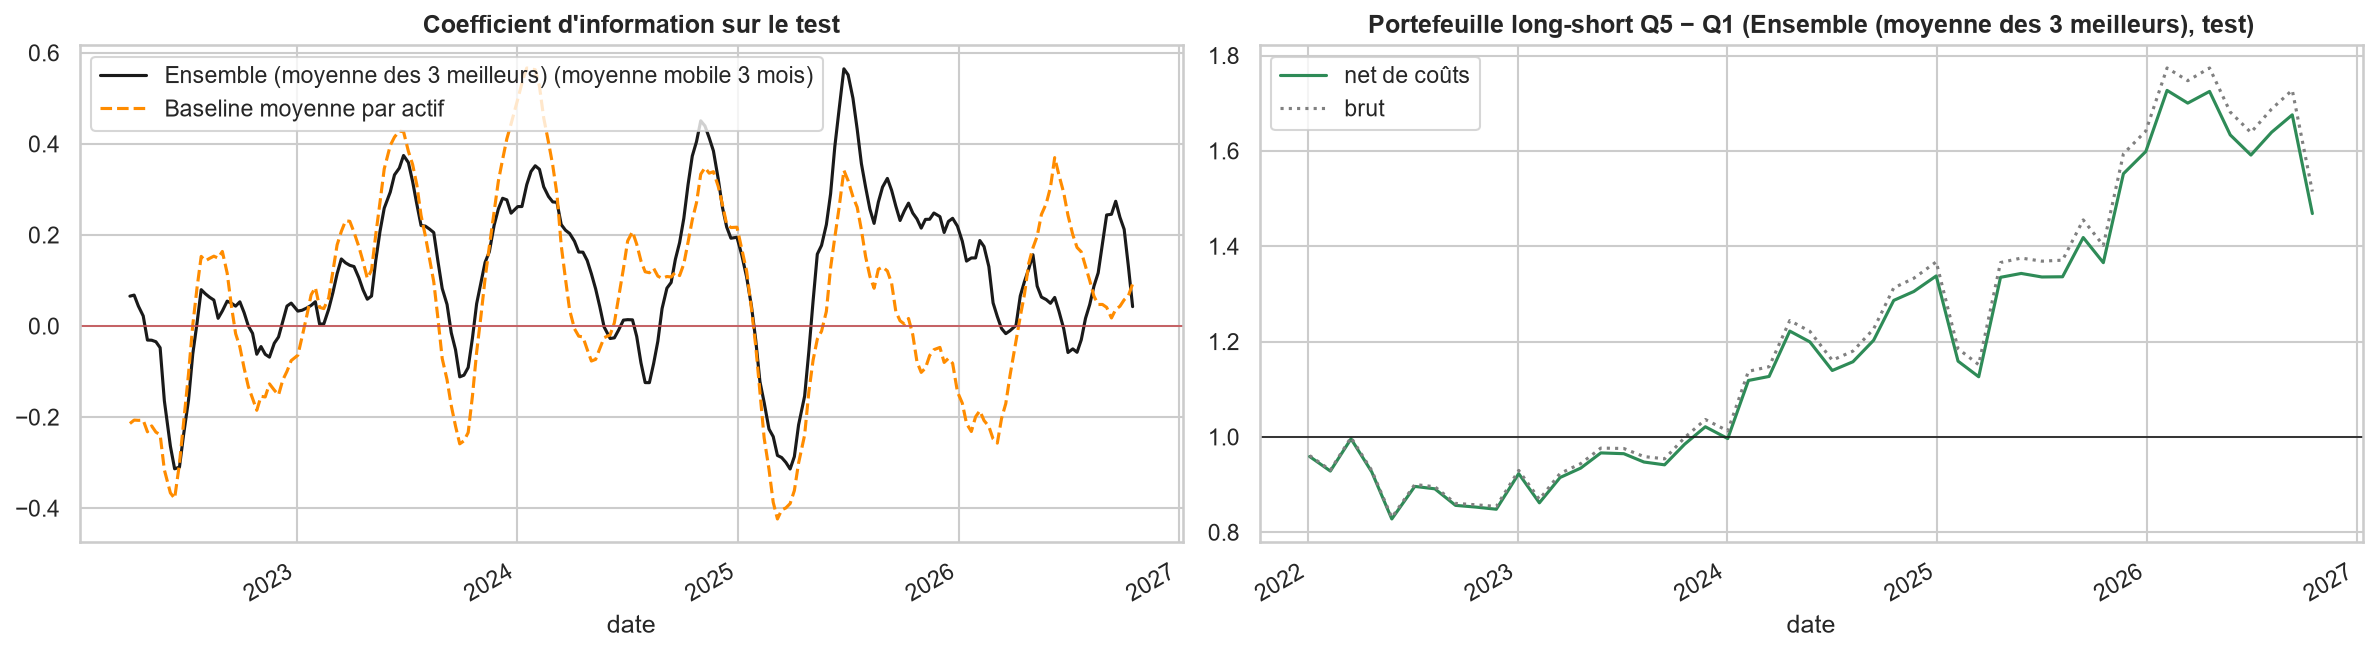
\includegraphics[width=\textwidth]{11_prevision_test.png}
  \caption{Sur le test : coefficient d'information (moyenne mobile sur trois mois) et valeur cumulée du portefeuille long-short Q5-Q1 construit avec l'ensemble.}
  \label{fig:prev_test}
\end{figure}

Ces résultats appellent trois commentaires.

\paragraph{La dérive des données s'est produite.} La référence \og moyenne par actif \fg{}, la meilleure sur 2013-2021, devient nettement moins bonne que la prévision nulle ($R^2 = -9{,}8$ \%). La prime de classe d'actifs s'est retournée en 2022, quand actions et obligations ont baissé ensemble. C'est exactement le risque annoncé par l'analyse exploratoire.

\paragraph{L'ensemble ne prévoit pas mieux les rendements.} Sa MSE est identique à celle de la prévision nulle ($R^2 = 0{,}15$ \%, $p = 0{,}94$). Le garde-fou a eu raison sur le critère qu'il s'était fixé.

\paragraph{Mais il classe un peu les actifs.} Son IC est de 0,10, significatif ($t = 2{,}35$), et le portefeuille long-short qui en découle gagne 9,8 \% par an après coûts. Faut-il en conclure qu'il aurait fallu l'activer ? Nous pensons que non, pour deux raisons. D'abord, l'IC a été très instable (négatif en 2022, autour de 0,17 de 2023 à 2025, proche de zéro en 2026) ; le simple momentum 12-1, sans apprentissage, fait presque aussi bien (9,4 \%). Ensuite, et surtout, changer la règle \emph{après} avoir vu le test reviendrait à utiliser le test pour décider : c'est précisément la fuite que tout notre protocole cherche à éviter. Le résultat est noté comme une piste : un critère fondé sur le classement (l'IC) plutôt que sur l'erreur quadratique pourrait être plus adapté à l'usage qu'on fait des prévisions. Il faudrait le valider sur une nouvelle période.

\subsection{Explicabilité et analyse des erreurs}

Les variables qui comptent le plus dans les prévisions (valeurs SHAP moyennes sur le test) sont les rendements passés à 3, 6 et 12 mois, le momentum 12-1 et les volatilités à 1 et 3 mois : le modèle combine un effet de tendance et un effet de risque. L'analyse par classe d'actifs montre que le modèle prévoit le bon \emph{sens} des écarts (rendement excédentaire prévu négatif pour les obligations et le monétaire, positif pour les actions et le Bitcoin) mais avec une amplitude bien plus faible que la réalité. C'est le comportement attendu d'un modèle fortement régularisé : il ramène ses prévisions vers zéro faute de confiance dans le signal.

En résumé, l'agent Prévision a été construit avec soin, évalué honnêtement et désactivé par une règle décidée à l'avance. Ce résultat négatif est, à nos yeux, l'un des apports du projet : il montre qu'un système d'apprentissage automatique doit savoir \emph{renoncer} à une prévision quand rien ne prouve qu'elle est utile.

